% !TEX root = ./Thesis - combined.tex

\chapter{An NMR compatible on-chip Peristaltic Pump}\label{Chapter:Peristaltics}

\section{Introduction}

The flow and control of liquids in microfluidics is essential, with microfluidic pumping
and mixing playing an integral role in many biological and chemical applications, such as
DNA analysis \citep{RN74, RN75}, protein folding \citep{RN76}, enzyme asssays \citep{RN77, RN78},
chemical synthesis \citep{RN79,RN80}, and kinetic studies \citep{RN81, RN82}. Many solutions to
the challenge of pumping and mixing at small scales exist, these include 3D printed valves \citep{RN83, RN84},
syringe pumps \citep{RN85,RN86,RN87}, pressure actuated valves \citep{RN88, RN89, RN90}, electrowetting
(sometime referred to as digital microfluidics) \citep{RN91, RN92}, piezoelectric pumps \citep{RN93, RN94},
magnetic pumping \citep{RN95,RN96}, and centrifugal forces \citep{RN97, RN98, RN99}.

In this chapter, the design and implementation of an NMR compatible, low dead volume,
microfluidic pump will be discussed. The aim of device is to be able to mix two fluids in a
controlled manner inside an NMR magnet. It will involve having an on-chip reservoir that
can be drawn from and mixed with whichever liquid that is under investigation. These aims
are important as the technology could be useful in chemistry applications such as a chemical
reaction study, kinetics study, or hyperpolarization on chip. The pump could be used in
biological studies too, with protein binding studies already being shown to be possible \citep{RN26},
these pumps could enable whole experiment to be performed on chip. Cell and living tissue
culture could also benefit from perfusion provided by the pump, supplying them with fresh O$_2$
and nutrients. Ultimately, the goal is to observe active changes on the chip, induced by
pumping, in real time, using NMR.

\begin{figure}
\begin{center}
  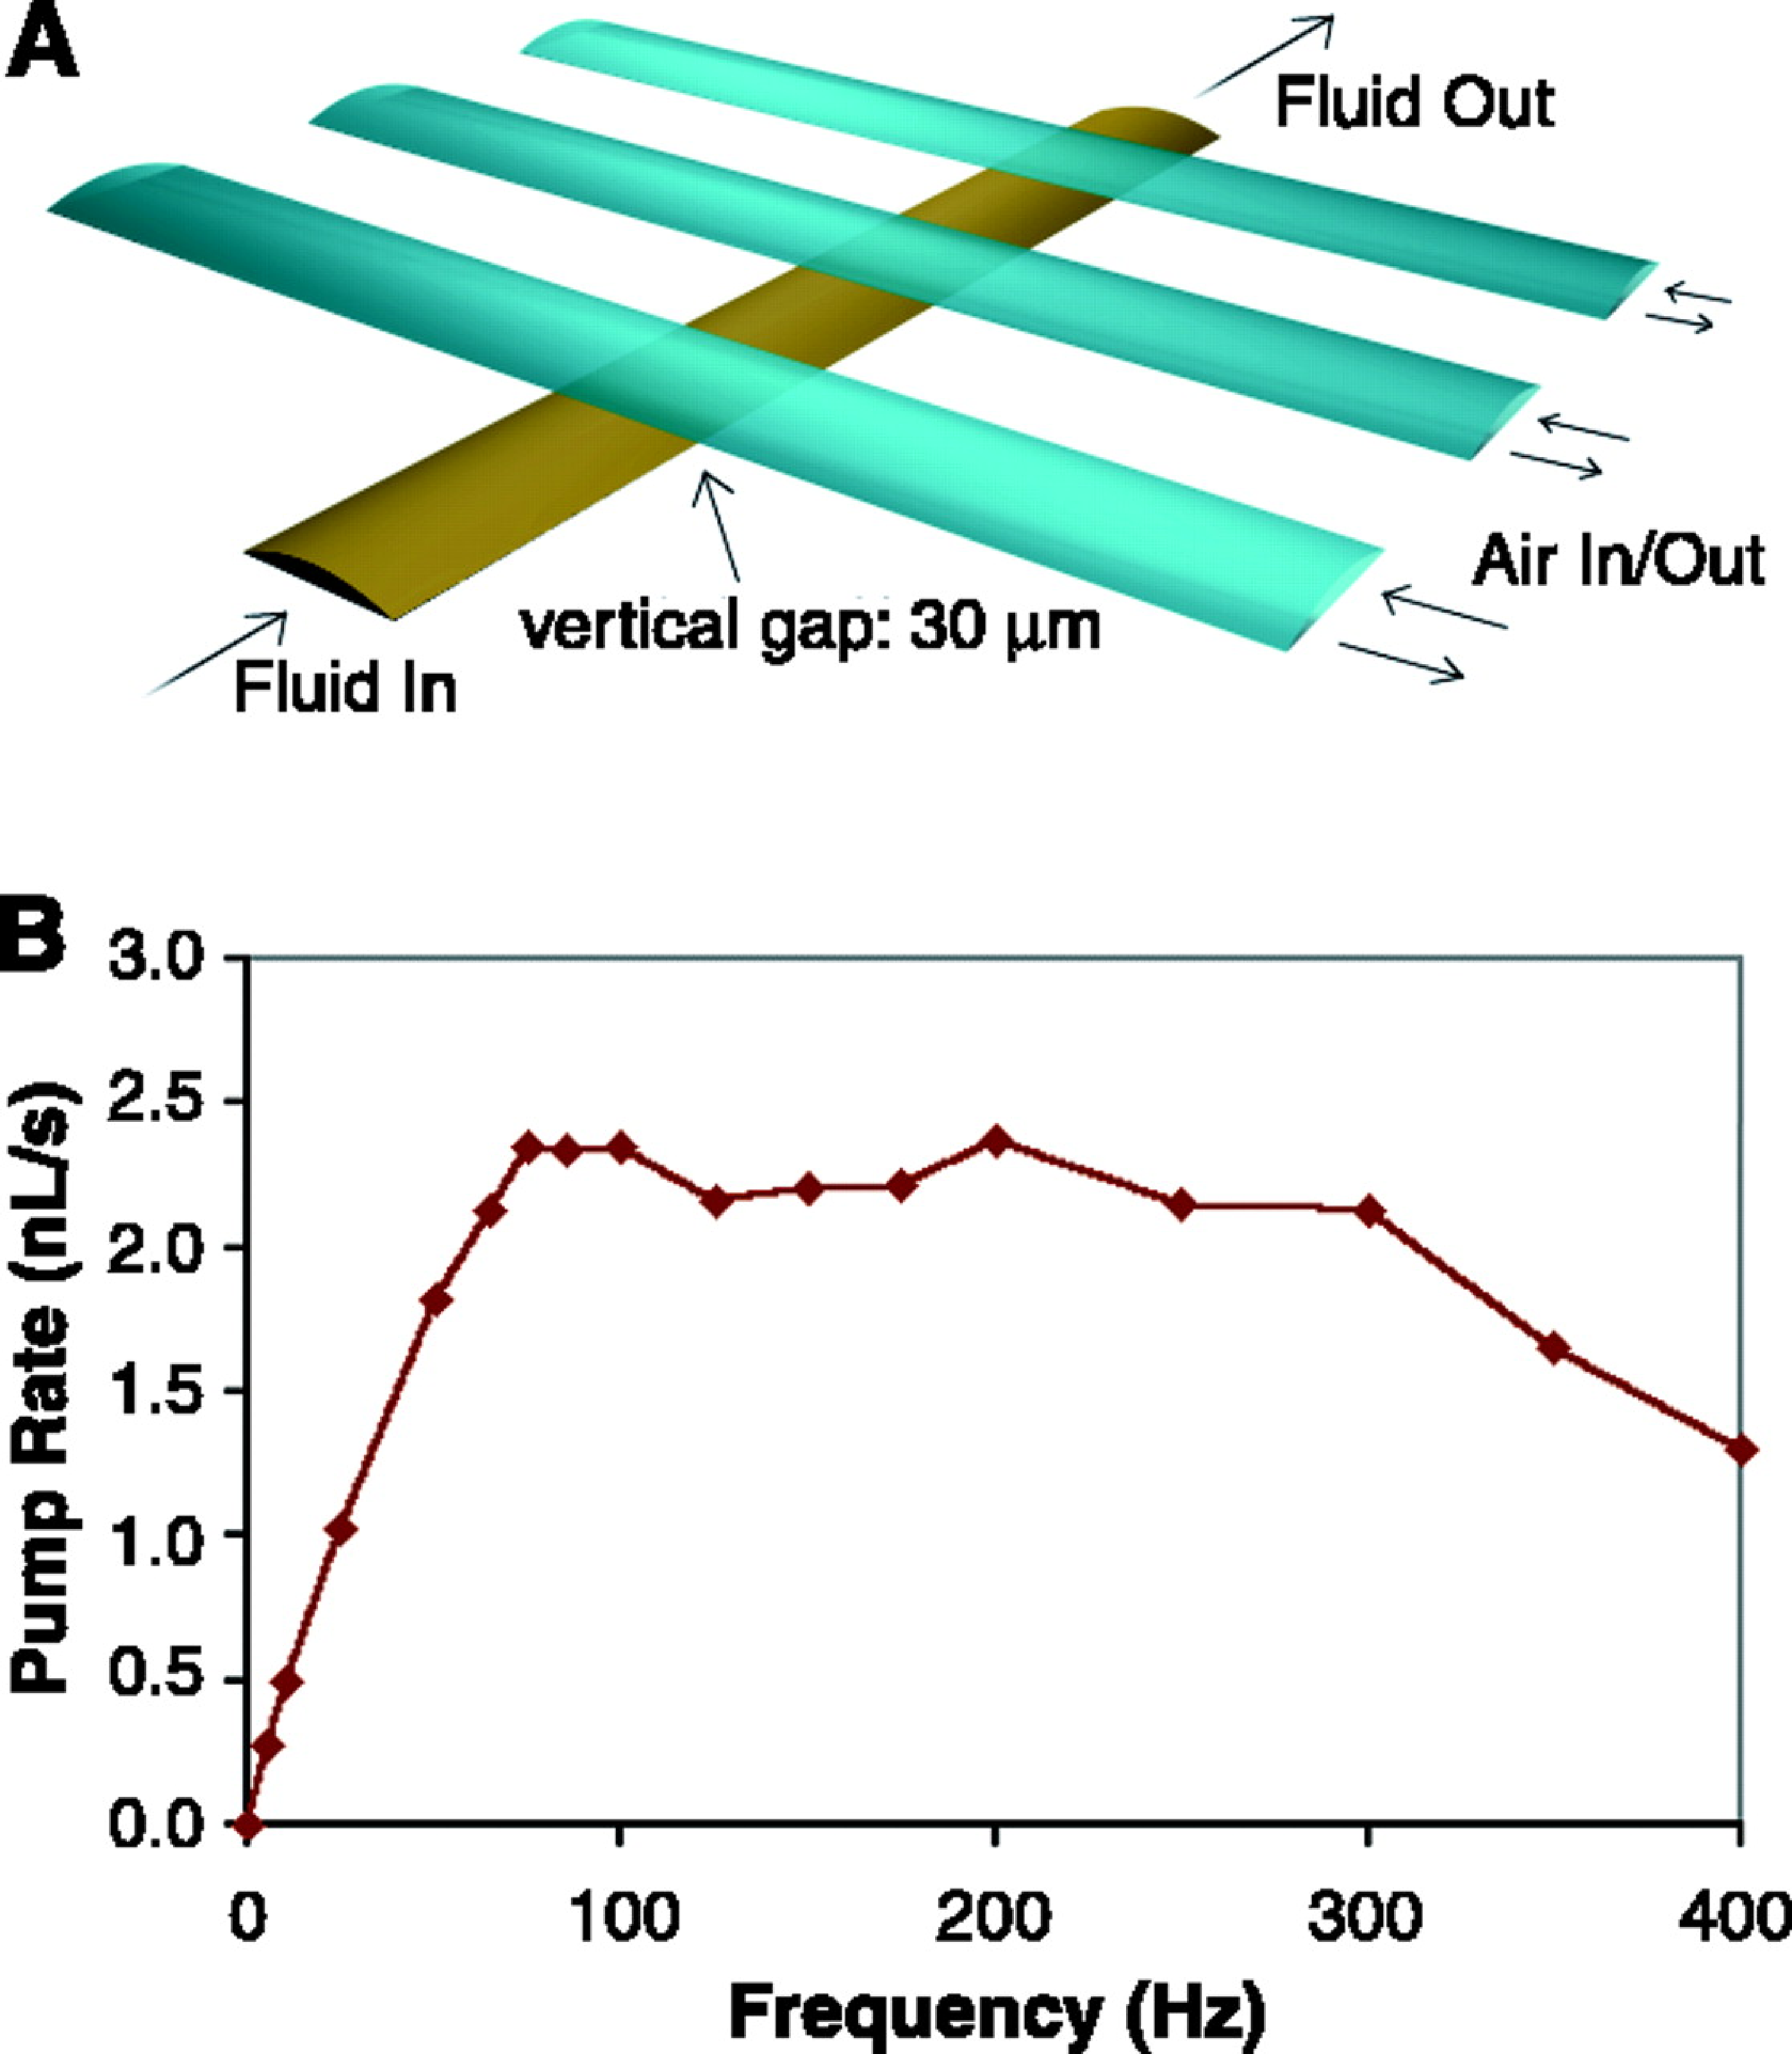
\includegraphics[height=10cm,keepaspectratio]{UngarFig.png}
\end{center}
  \caption{A) A 3D scale diagram of an elastomeric peristaltic pump. The channels are 100 μm wide and 10 μm high.
  Peristalsis was typically actuated by the pattern 101, 100, 110, 010, 011, 001, where 0 and 1 indicate “valve open”
  and “valve closed,” respectively. B) Pumping rate of a peristaltic micropump versus various driving frequencies. This
  figure is reproduced from \citep{RN59}.}
  \label{fig:Ungar}
\end{figure}

Pumps that integrate pumping ‘on chip’ are key to minimising the dead volume within the device.
Unger and co-workers \citep{RN59}, were amongst the first to do this by micro-fabricating PDMS valves
using soft lithography. \fig{fig:Ungar} shows the devices, these work by having a central fluid path that has various gas
channels running perpendicular above it. By simply applying air pressure, the gas channel expands cutting off
the flow in the fluid path beneath. When these valves are actuated in sequence, they produce a
net movement of fluid and flow rates of 2.5 nL/s were achieved.

Leslie et al \citep{RN100} had slightly different
approach. In the ‘pump’ the PDMS forms
a dome above a circular structure in the fluid channel that is the depressed using air
pressure. In order to control the flow they use so called fluidic diodes, these work
analogously with electric diodes, by only allowing fluid flow above a certain pressure in
one direction only. These diodes are formed by having a weir that separates two fluid
channels covered by a compliant PDMS membrane. When the internal fluid pressure reaches the
threshold, this pushes the PDMS membrane up and allows fluid connection over the weir. The
pressure required to open the diode depends on the thickness of the PDMS ceiling and is
predictable which allowed control of flow in the chip at large.

\begin{figure}
\begin{center}
  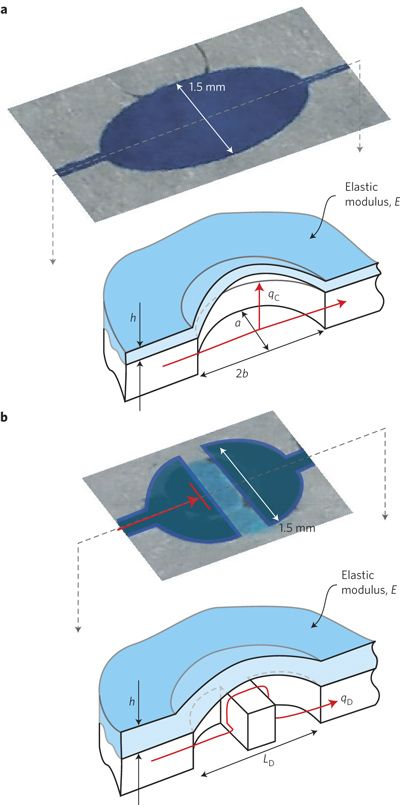
\includegraphics[height=12cm,keepaspectratio]{Leslie-Valves.jpg}
\end{center}
  \caption{\textbf{a}, Discrete fluidic capacitors are created by bonding deformable films (in
   this case, PDMS) over reservoirs placed in the network between fluidic channels (resistors)
    fabricated in glass. These features store and release fluid (volumetric flow rate, qC) in
    proportion to the time rate of change in pressure inside the network; the proportionality
    constant (capacitance, C) depends on film thickness (h), span (a, b) and elastic modulus
    (E). \textbf{b}, Discrete fluidic diodes are created by bonding deformable films around
    weirs that separate two channels in the network. When the internal pressure is larger than
    the external pressure, the diode opens and exhibits nonlinear pressure–flow relationships
    (volumetric flow rate, qD) dictated by solid–fluid coupling. When the internal pressure is
    less than the external pressure, the diode pulls shut and prevents flow. Figure taken from
    \citep{RN100}.}
  \label{fig:Ungar}
\end{figure}

There are specific challenges related to enabling on-chip pumping in a high magnetic field to perform high
resolution NMR spectroscopy. Firstly, the materials used should be compatible with a high
magnetic field clearly ruling out ferrous metals, this also rules out materials that
have a significantly different magnetic susceptibility to that of the chosen fluid (in this
case water). As described in chapter \ref{Chapter:Droplets}, susceptibility mismatches need to be carefully
managed, or they will interfere with the homogeneity of the magnetic field which
essential for production high resolution spectra. Secondly, materials chosen must also be
conducive to rapid prototyping, and as such must be cheap and readily available as well as
be easily cut by a laser cutter and bonded using a simple method. These reasons rule out
glass, a common microfluidic material, which is not easily cut using a standard
laser cutter. Thirdly the chip, when fully assembled, should not be more
that 1 mm in thickness, due to limitations imposed by the strip-line probe geometry \citep{sharma2019modular}. This
limitation  means that more brittle materials, such as glass, would be too fragile for
continuous insertion into the probe and magnet. Lastly,
the device should be able to seal against gas and liquid pressures whilst in operation
inside the magnet.

With all these limitations, poly(dimethylsiloxane) (PDMS) would seem an ideal candidate. It is: cheap and
readily available; easy to cut and bond; and can but made into 1 mm layers to fit the
transmission line probe. However, due to its amorphous structure the $^1$H background
signal is large and broad across the range of ppm that the signals that we are interested in
appear. This broad background signal makes it impractical to suppress and any suppression would also suppress the
signals that we are interested in, and could lead to difficulties in quantification of
substances present in the sample under investigation.

In the design shown, a PDMS layer is still used. However, it is removed from the
sensitive area around the sample chamber so that it does not interfere with the signal
collected from the device. The 3D printed parts role here is three-fold, firstly, it acts
as a conduit for delivering liquids and transporting them around the device. Secondly, it
allows for the pressurised air to be delivered which drives the pneumatic valves and
enables pumping. Lastly, when screwed together, the 3D printed parts form a seal against
liquid and gas leaks.

Nuclear magnetic resonance (NMR) is an ideal tool with which to study live systems,
which owing to its non invasive non destructive nature, can give insight into living
systems \textit{in situ} and allows for longitudinal studies of them. However, in order to
keep these systems alive, and truly replicate \textit{in vivo} conditions, they need fresh supplies of oxygen and nutrients. One way of achieving this is by perfusion of
liquid that has been exposed to fresh supplies of oxygen. Perfusion can be accomplished by
pumping liquid through the microfluidic device and then out to a reservoir that is in
contact with a supply of oxygen. This method would, however, dilute any metabolites
given off by the living system that is under investigation within the device, and
since the biggest limitation of NMR is sensitivity, it is pertinent to avoid this. This
means that the pump would ideally be integral to the device itself. This could reduce the
overall volume of the system to tens of microlitres which is much better than the tens of
millilitres that come from having an external pumping network. This means that the pump
would ideally be integral to the device itself.

In summary, the device must meet the following criteria:
\begin{itemize}
  \item Non-magnetic parts where possible, susceptibility matched.
  \item Easily fabricated using rapid prototyping.
  \item Low dead volume.
  \item Biocompatible.
  \item Geometry compatible with transmission line probe.
  \item Easily assembled and operated \textit{in situ}.
\end{itemize}

The solution employed here involves a multilayered PMMA device,
with two PDMS membranes, sandwiched between two 3D printed holders held together with brass
screws. The PMMA device houses the structures for the valves, as well as the fluid circuits,
including an NMR sensitive sample chamber and on-chip reservoir. The PDMS layers have two
separate functions, the top membrane forms the valves with the PMMA structures whilst the
bottom membrane acts as an o-ring to seal against fluid leaks. The 3D printed holders
are also multi purpose. The top holder forms the last part of the valves by sealing the
PDMS-PMMA valve and allowing the delivery of pneumatic pressure through the bore of the
magnet to the device. The bottom 3D printed holder allows the device to be filled and
supplies external ports for fluid short circuiting. Together, they help seal the device
against gas and liquid leaks. This device coupled with a bespoke, homebuilt probe enables
pumping and observation by NMR in a microfluidic device.

\subsection{Materials and Methods}

The devices are composed of three layers of cell cast poly(methyl methacrylate) (PMMA,
Weatherall Equipment). The sheet thickness was 200 $\mu$m for the top and bottom layers, and 500 $\mu$m for
the middle layer. The channels and sample chambers were designed in
AutoCAD and cut using a CO$_2$ laser (HPC Laser ltd.) to an approximate width and depth
of 150 $\mu$m. These layers were bonded together using plasticiser (2.5\% v/v dibutyl
phthalate in isopropyl alcohol) and subjected to heat and pressure (358 K, 18.6 MPa).
To seal the devices, two polydimethyl siloxane (PDMS, Shielding Solutions) were
designed in AutoCAD and cut using the same laser as the PMMA layers.

The PMMA and PDMS were screwed together and held in place using 3D printed devices
designed in SolidWorks (Acura Xtreme, ProtoLabs). These, as shown in \fig{fig:3Ddevice}, seal the
device whilst enabling the filling of the device as well as delivering the pressurised
air for the peristaltic pumping.

The hardware for controlling pumping comprised of a solenoid valve system with 8
individual valves (Festo, RS). These were connected to 3mm plastic tubes (Festo, RS)
and all supplied from an in-lab air pressure source. This valve system was connected,
via a solderless breadboard, to an arduino (Mega 2560, RS) controller allowing for
individual control of each of the valves. The Solenoid valve system was powered using
a 24V supply.

The device was put into a transmission line based home-built probe. In this, the
device is held between two striplines with the inner sample chamber lining up with the
constriction on the strip-lines. NMR measurements were performed on a bruker AVANCE
III spectrometer and 11.7 T magnet. Spectra were collected using 64 scans using a 90
degree pulse length of 2.5 us at 50 W of power. Water suppression was achieved by
using presaturation with $5x10^{-4}$ W.

100mM solutions of sodium acetate (Merck) and 3-(Trimethylsilyl)-1-propanesulfonic
acid (DSS, Merck) by dissolving 82 mg and 196 mg in 10 ml of deionised water
(ReAgent)
respectively. The two fluidic loops were then filled with these separately and the
in/out ports short circuited.

Firmware for controlling the peristaltic pump was written in Arduino and is provided in the appendix.
This has the ability to put the pump into 3 states
“advance”, “mixing” and “quiet”. The “advance” state pumps from the outside loop of
the device to the inside loop for a desired number of seconds; “mix” pumps around the
inner loop for a desired number of seconds; and “quiet” stops all pumping and leaves
all valves open indefinitely.

\begin{figure}[h]
  \begin{center}
  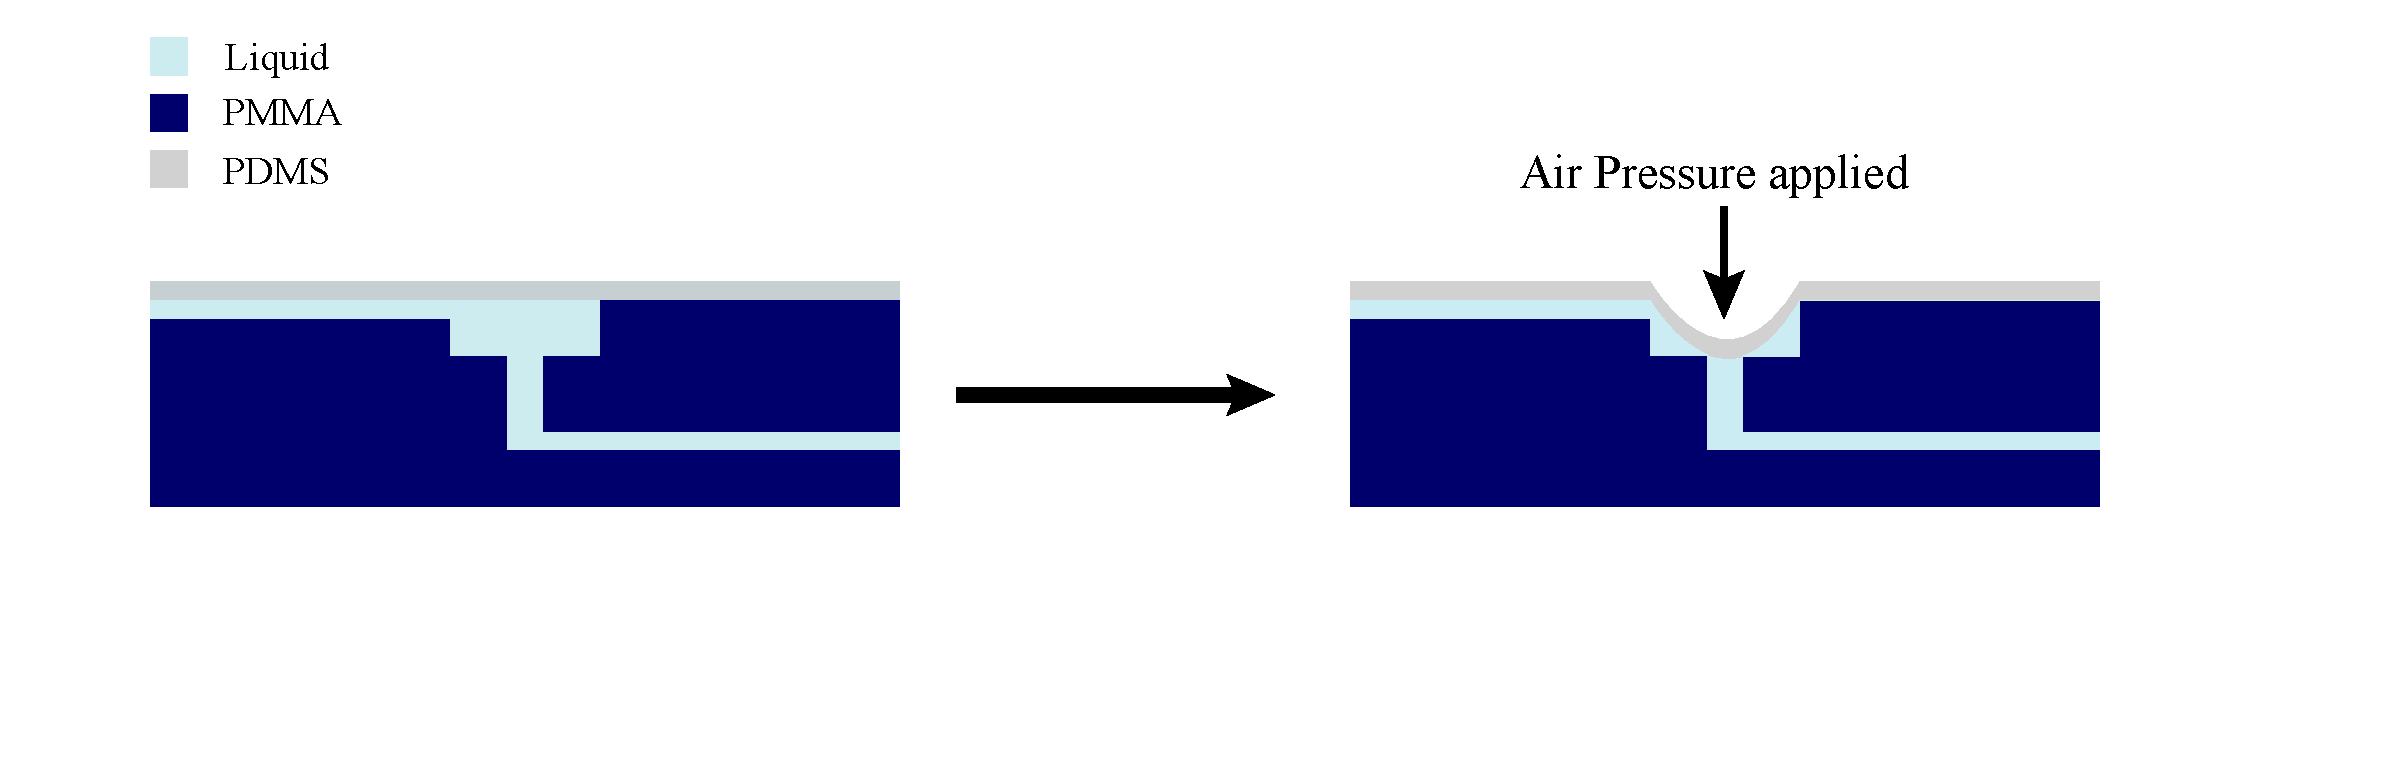
\includegraphics[width=\columnwidth]{Peristaltic-principle.pdf}
  \caption{A cut-through view of the valves in the device showing how when air pressure is
  appplied the PDMS membrane is pushed down and seals the small hole cut in the middle layer.}
  \label{fig:PP-device}
  \end{center}
\end{figure}

\begin{figure}[h]
  \begin{center}
  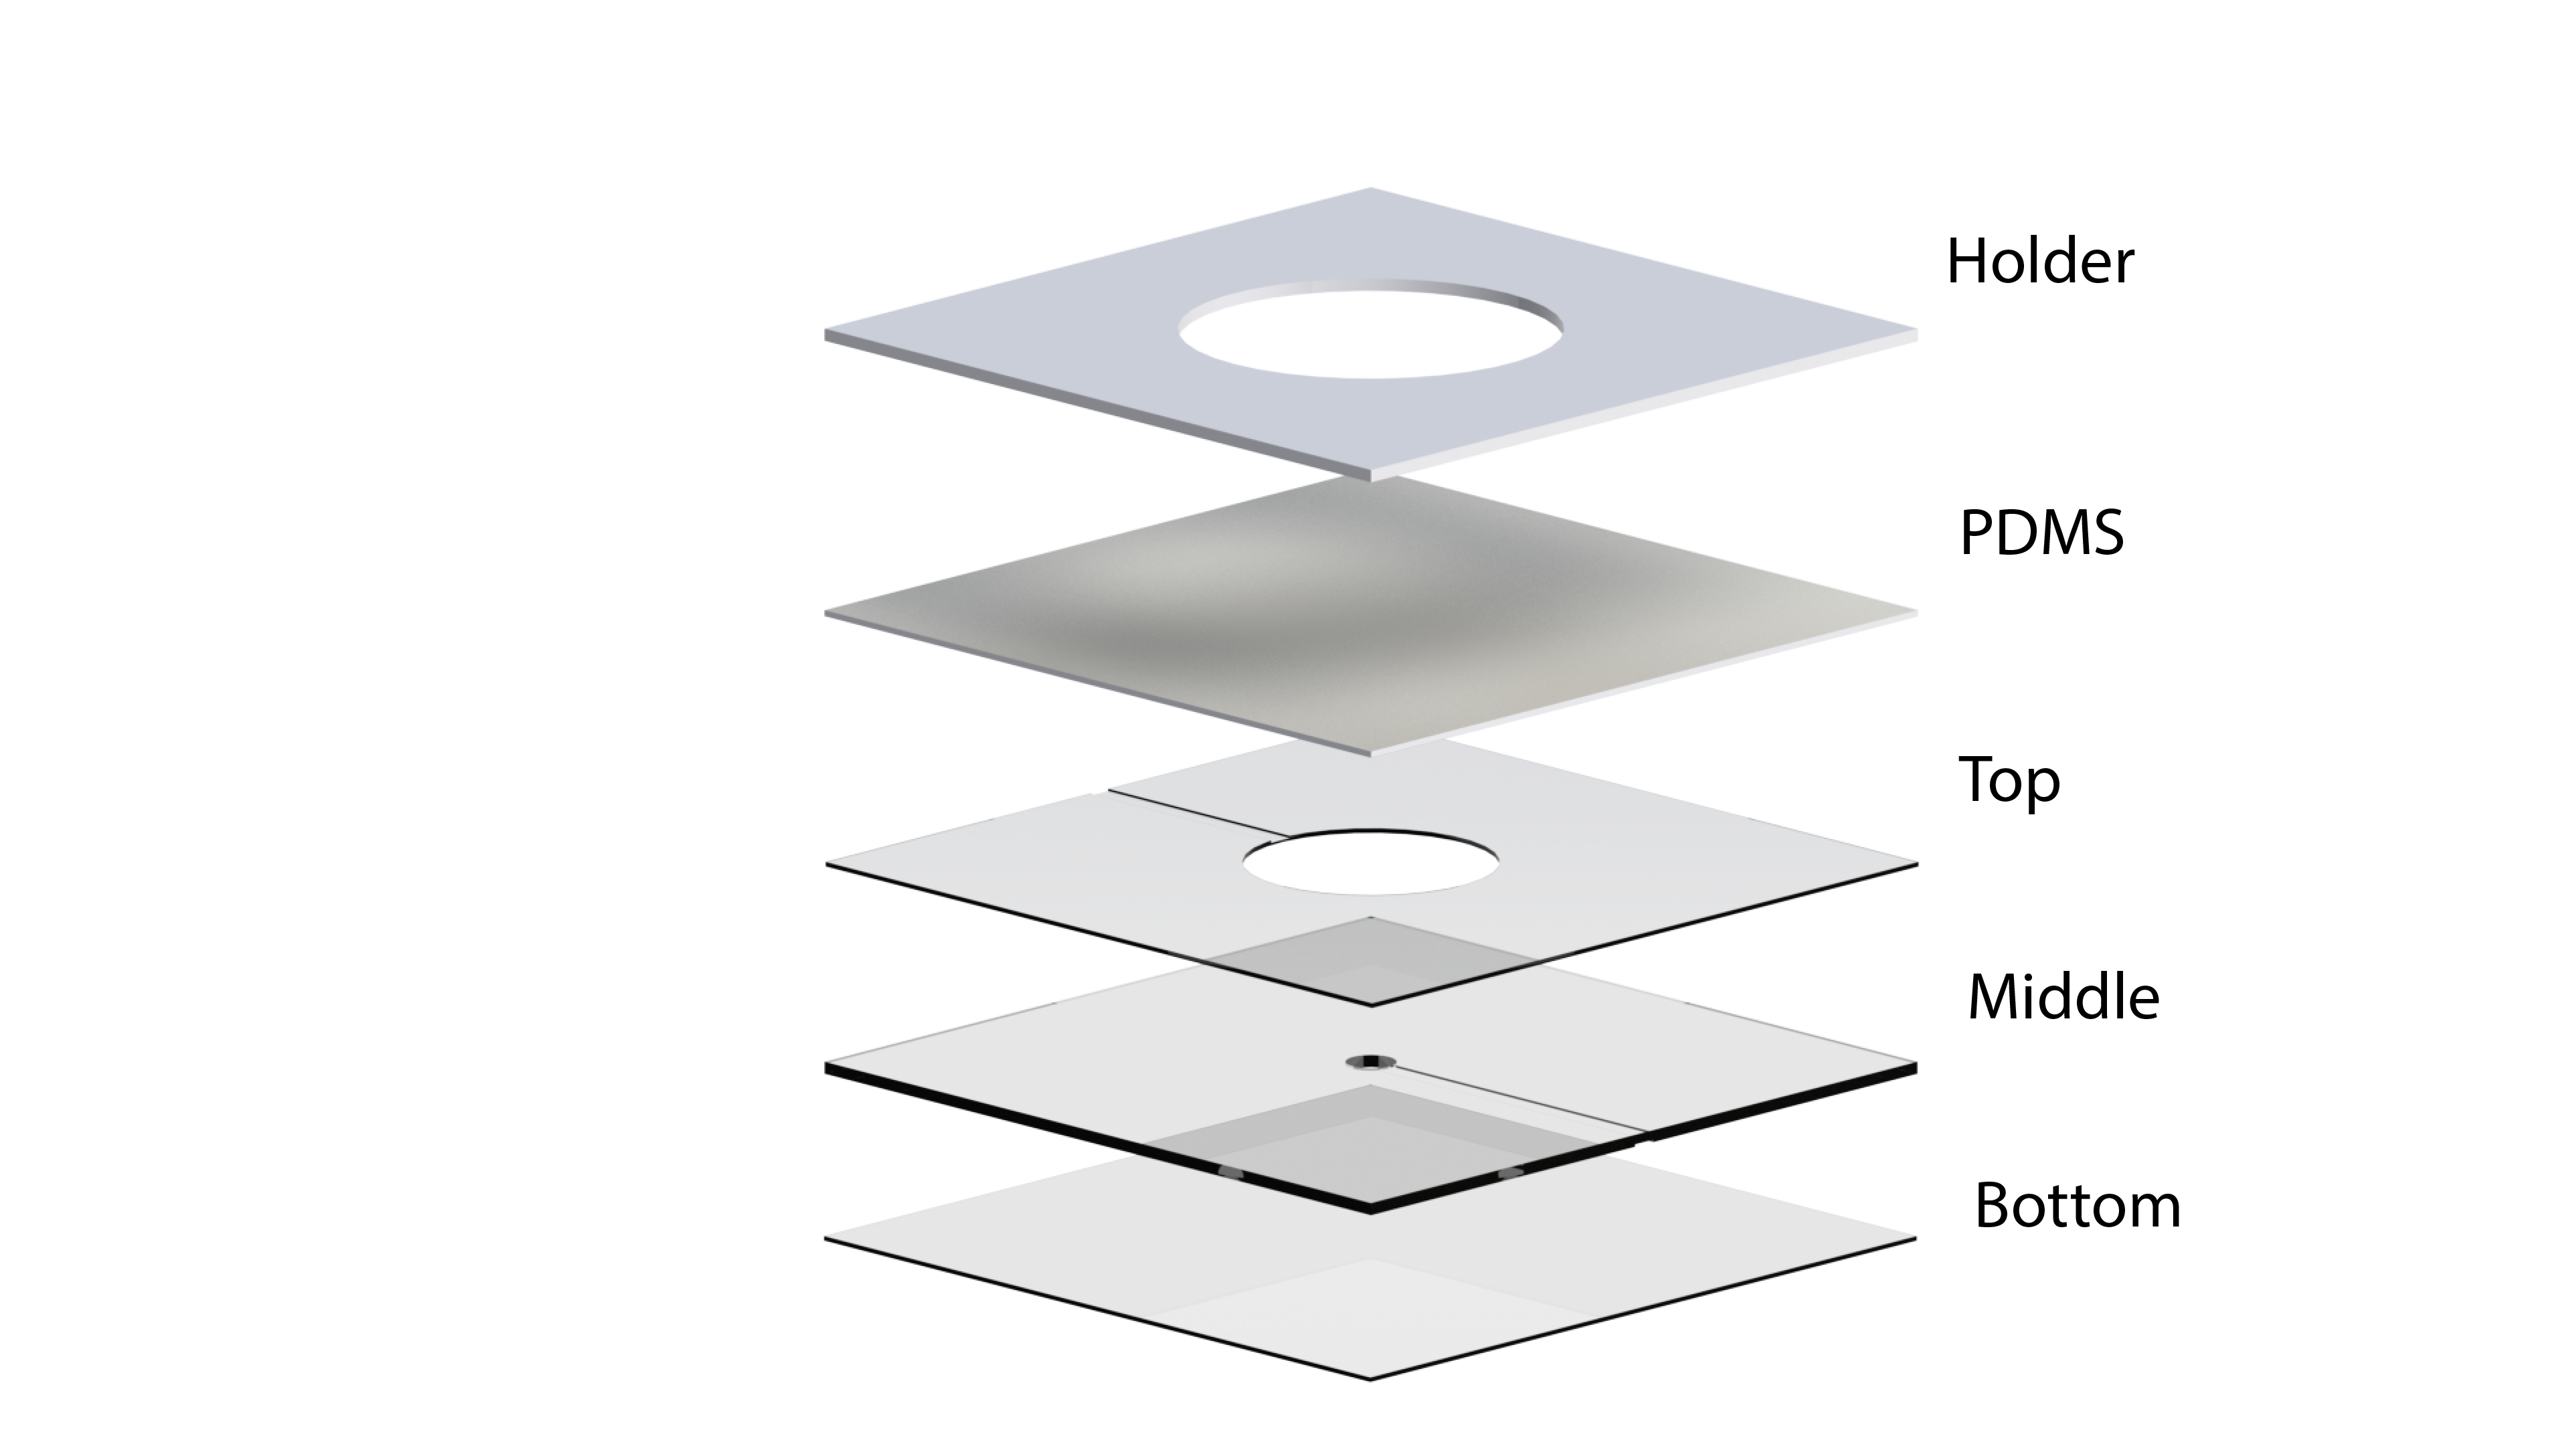
\includegraphics[width=\columnwidth]{3DRenderOfValve-01.png}
  \caption{3D render of a single valve with 3D printed layer shown too}
  \label{fig:ValveRend}
  \end{center}
\end{figure}

\section{Results and Discussion}

\subsection{Peristaltics}

In order for the dead volume in the device to be kept at a minimum, the valves are implemented
in the fluid path on the device itself. Shown below in \fig{fig:PP-device} is the
basic principle behind the design.

\begin{figure}[h]
  \begin{center}
  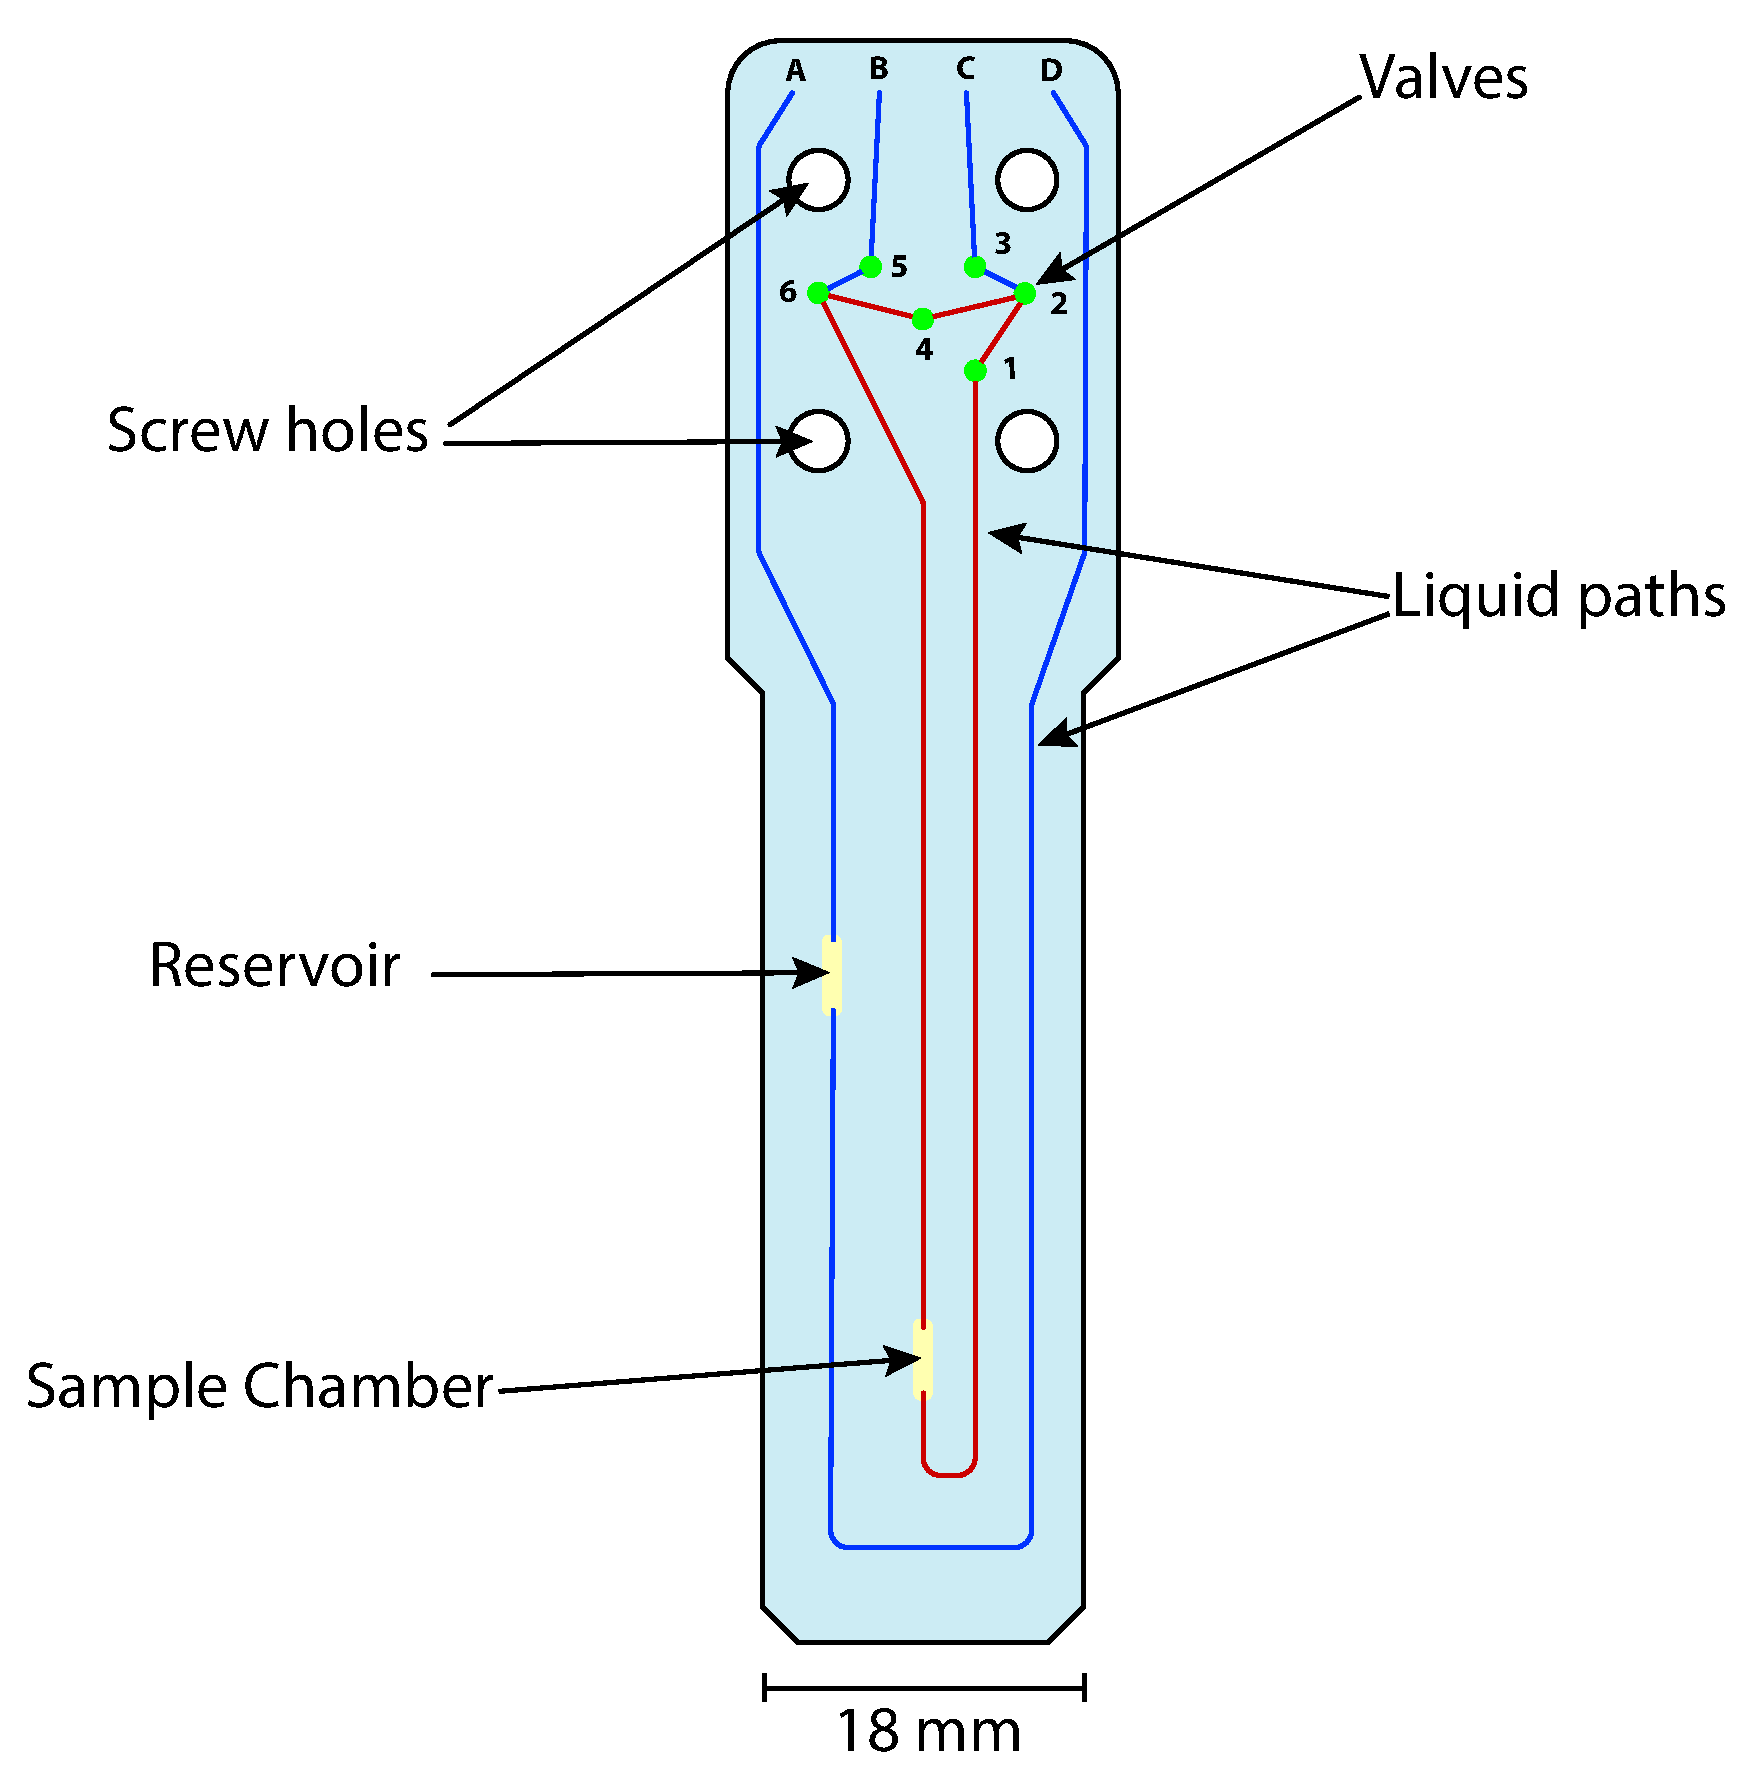
\includegraphics[width=\columnwidth]{Experimental-chip.pdf}
  \caption{A CAD drawing of the chip designed for pumping and mixing. Inner (red) and outer (blue) liquid circuits; liquid ports (\textbf{A}-\textbf{D}) and valve positions (1-6) shown.}
  \label{fig:Chip}
  \end{center}
\end{figure}

In the device, there are valves cut into the layers of PMMA. These are formed by two holes
in the top and middle layer. The hole in top layer has a radius of $500 \mu m$ whilst the
hole in the middle layer has a radius of $100 \mu m$. The top layer has a channel (approx.
$150\mu m$ in width and depth) scored into it to deliver fluid to the top chamber whilst
the middle layer
has a similar channel scored on the under-side to carry fluid away. When covering the hard
PMMA structure with the more compliant PDMS membrane of $250 \mu m$ thickness, applying
air pressure from above seals the valve by covering the hole in the middle layer.

\begin{figure}[h]
  \begin{center}
  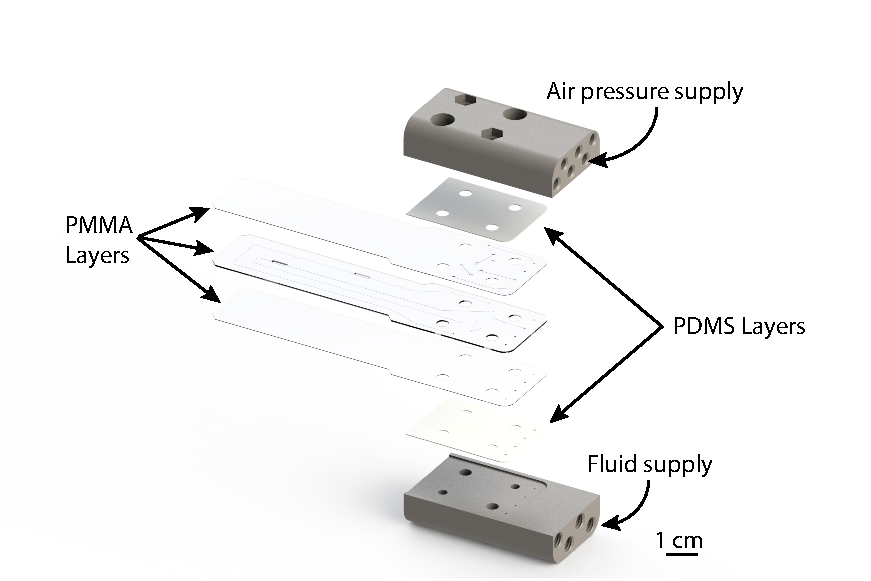
\includegraphics[width=\columnwidth]{Peristaltic-Chip-Render-01.pdf}
  \caption{A 3D representation of the device with separate layers of chips and PDMS
  layers shown.}
  \label{fig:3Ddevice}
  \end{center}
\end{figure}

A 3D rendering of a single valve is shown in \fig{fig:ValveRend} and shows the ratio of pump holder opening, top hole; and middle hole respecively. The key to these valves
is that the scored channels are on opposing sides of the valve.

\begin{figure}[h]
  \begin{center}
  \includegraphics[width=\columnwidth]{Micrographs-02.png}
  \caption{Micrographs of A: free chip showing two valves B: An assembled device with an
  open valve C: An assembled device with a closed valve, the arrows indicate the area where the PDMS is
  in contact with the PMMA and is sealing the hole.}
  \label{fig:Micrographs}
  \end{center}
\end{figure}


In \fig{fig:Micrographs}, micrographs of the chip outside the holders are shown with the valves
where one can see the fluid channels on opposing side of their respective layers. Also given,
is side by side comparison of the same valve (valve 2 in \fig{fig:Chip}) open (2) and closed
(3) one can see the 'ring' formed by the PDMS as it seals against the middle layer.

In my design, there are 6 such valves all individually addressable with air pressure, which when
coupled with home-written Arduino firmware, can be actuated in sequence in order to move
fluid in a given direction. The block diagram of the arduino set-up is shown in
\fig{fig:ValveSetup}. By varying the frequency and lambda parameters, listed in the
firmware, one can control the liquid pumped in a given time.

\begin{figure}[h]
  \begin{center}
  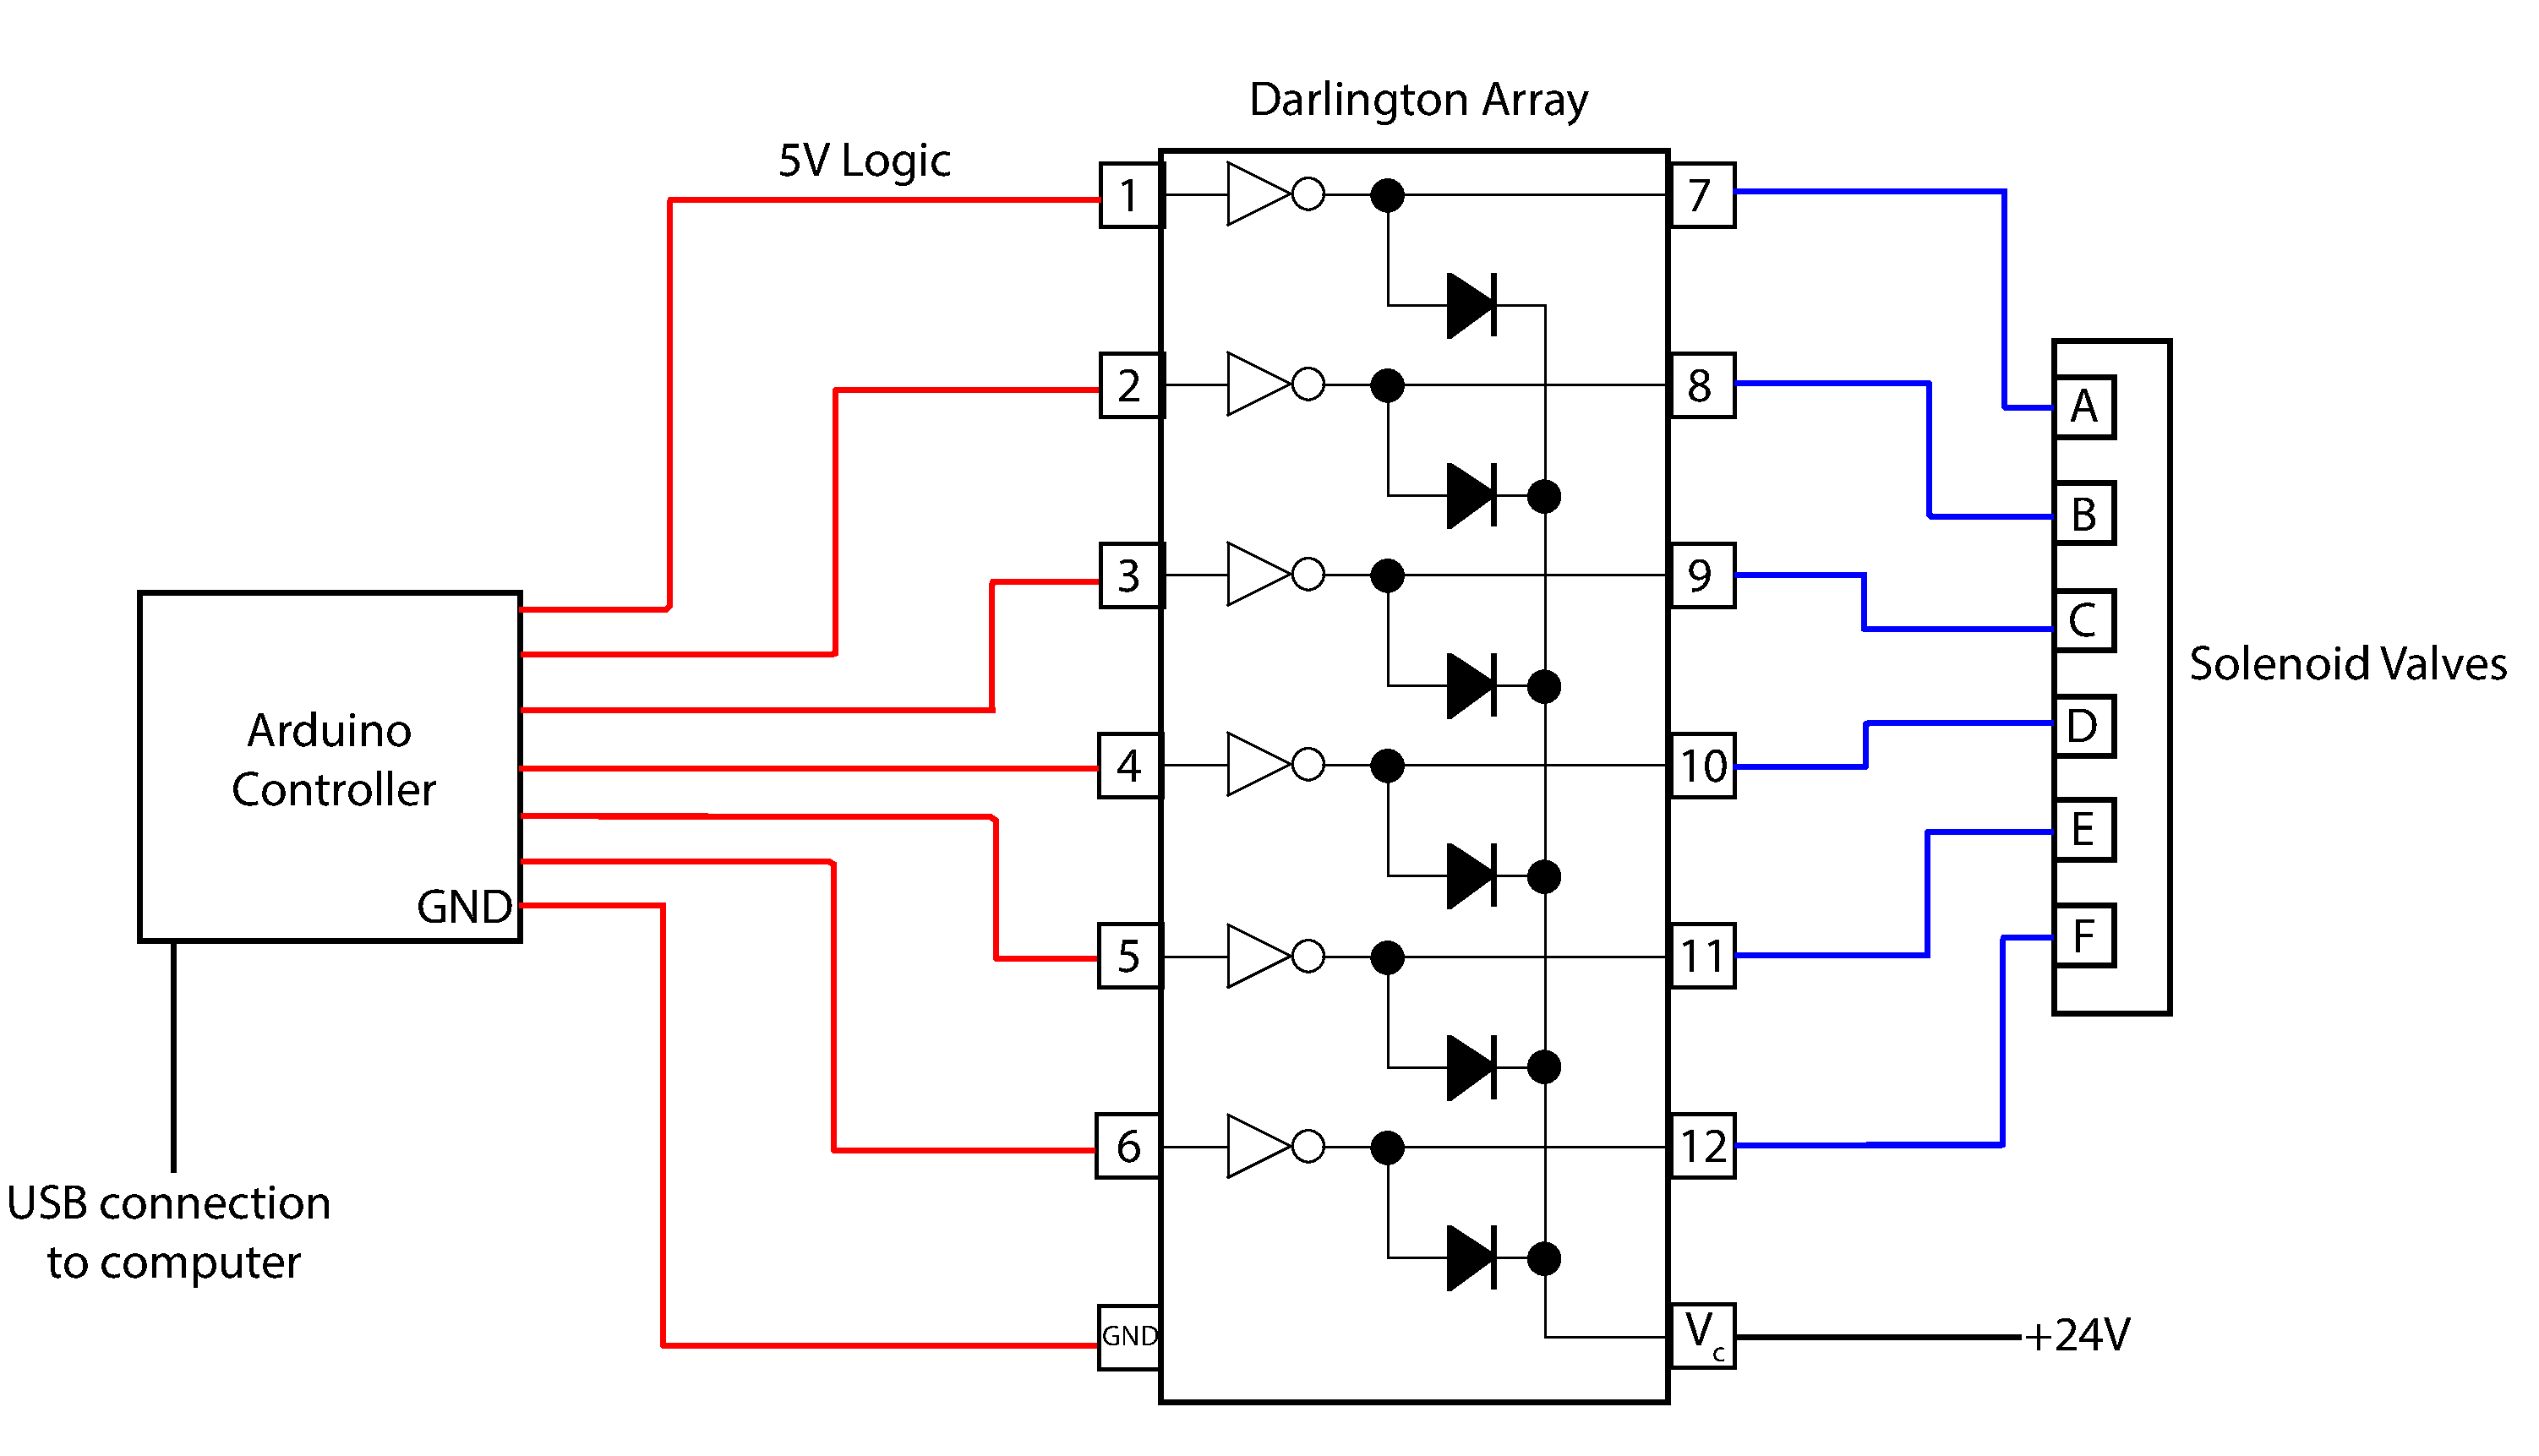
\includegraphics[width=\columnwidth]{Arduino-Valve.pdf}
  \end{center}
  \caption{An arduino controller is connected to, and powered by, a laptop via USB. The controller is connected
  to a darlington array via six 5V logic connections (shown in red) when addressed, these allow the corresponding pin
  opposite to draw power from the +24V connected from an outside source. The blue lines indicate the the wires
  carrying 24V to the solenoid bank which are pneumatically connected to the valves in the chip as labelled. }
  \label{fig:ValveSetup}
\end{figure}

As well as 6 valves, the chips also have two separate liquid
circuits that can be connected externally by attaching tubes to the top of the 3D
holders as shown in \fig{fig:Chip}. The inner circuit on
the diagram contains the pumping network which can be
modified to pump around the internal circuit or the complete network, and an NMR
sensitive sample chamber where measurements are performed. The external circuit,
contains an identical sample chamber that helps to keep the relative
volumes of the two circuits similar. The chip is filled from the
‘bottom’ using the 4 small access holes at the top of the chip (\textbf{A}-\textbf{D}).
This then allows the valve network and pressurised air to be
on the top side of the chip. The challenge in the chip was to fit
all the liquid paths and valve network around the 4 large
holes in the top of the design which accommodate the screws
necessary to hold the device together, and seal against leaks of
both liquid and gas.


\subsection{Characterisation of flow}

Characterisation of flow experiments where performed with the device in an “open”
configuration. This means that after the device was screwed together the two circuits shown
in blue and red were joined together by fixing tubing between the \textbf{A} and \textbf{B} ports shown in
\fig{fig:Chip}. This leaves \textbf{C} as the “in” port and \textbf{D} to be the “out” port with valves 3, 2, and 1
being actuated in sequence to pump, and valve 4 sealed.

The device was connected to translucent polytetrafluoroethylene (PTFE) tubing (Outer
diameter 1.6 mm, inner diameter 0.8 mm) with one end submerged in a 500 mL beaker
containing filtered DI water (Reagent). Next to the device a ruler was secured to the bench
top with the tubing fixed parallel to it. The pump was then switched on and the device
allowed to draw water, and pump out the other side. When the water meniscus reached the tubing
next to the ruler a timer was started and the distance along the ruler was recorded every
minute for 10 minutes. The was repeated 3 times for frequencies from 0.25-1 keeping the
lambda constant at 3, which had shown through trial and error to be the optimum number.

The graph shown in \fig{fig:Graph} is the result of plotting the cumulative volume pumped
vs. time. All 4 frequencies show very little deviation from linearity in the
long term and also show very small error bars (plotted as ±2$\sigma$).

\begin{figure}[h]
  \begin{center}
  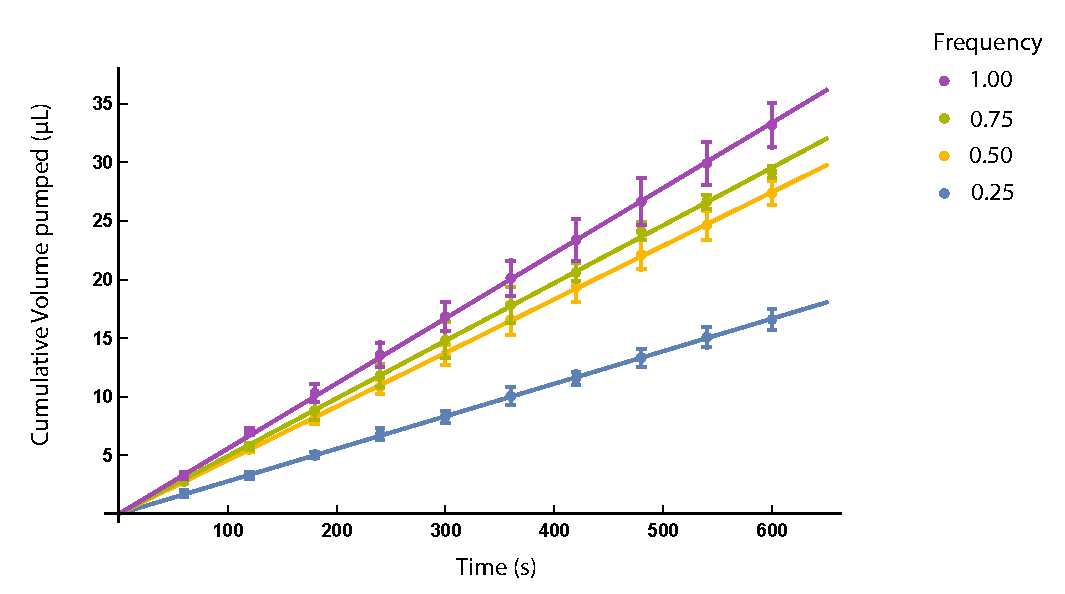
\includegraphics[width=\columnwidth]{ALLPlots.pdf}
  \caption{Plot of the total volume pumped vs time for a chip in the open
  configuration.}
  \label{fig:Graph}
  \end{center}
\end{figure}

\begin{figure}[h]
  \begin{center}
  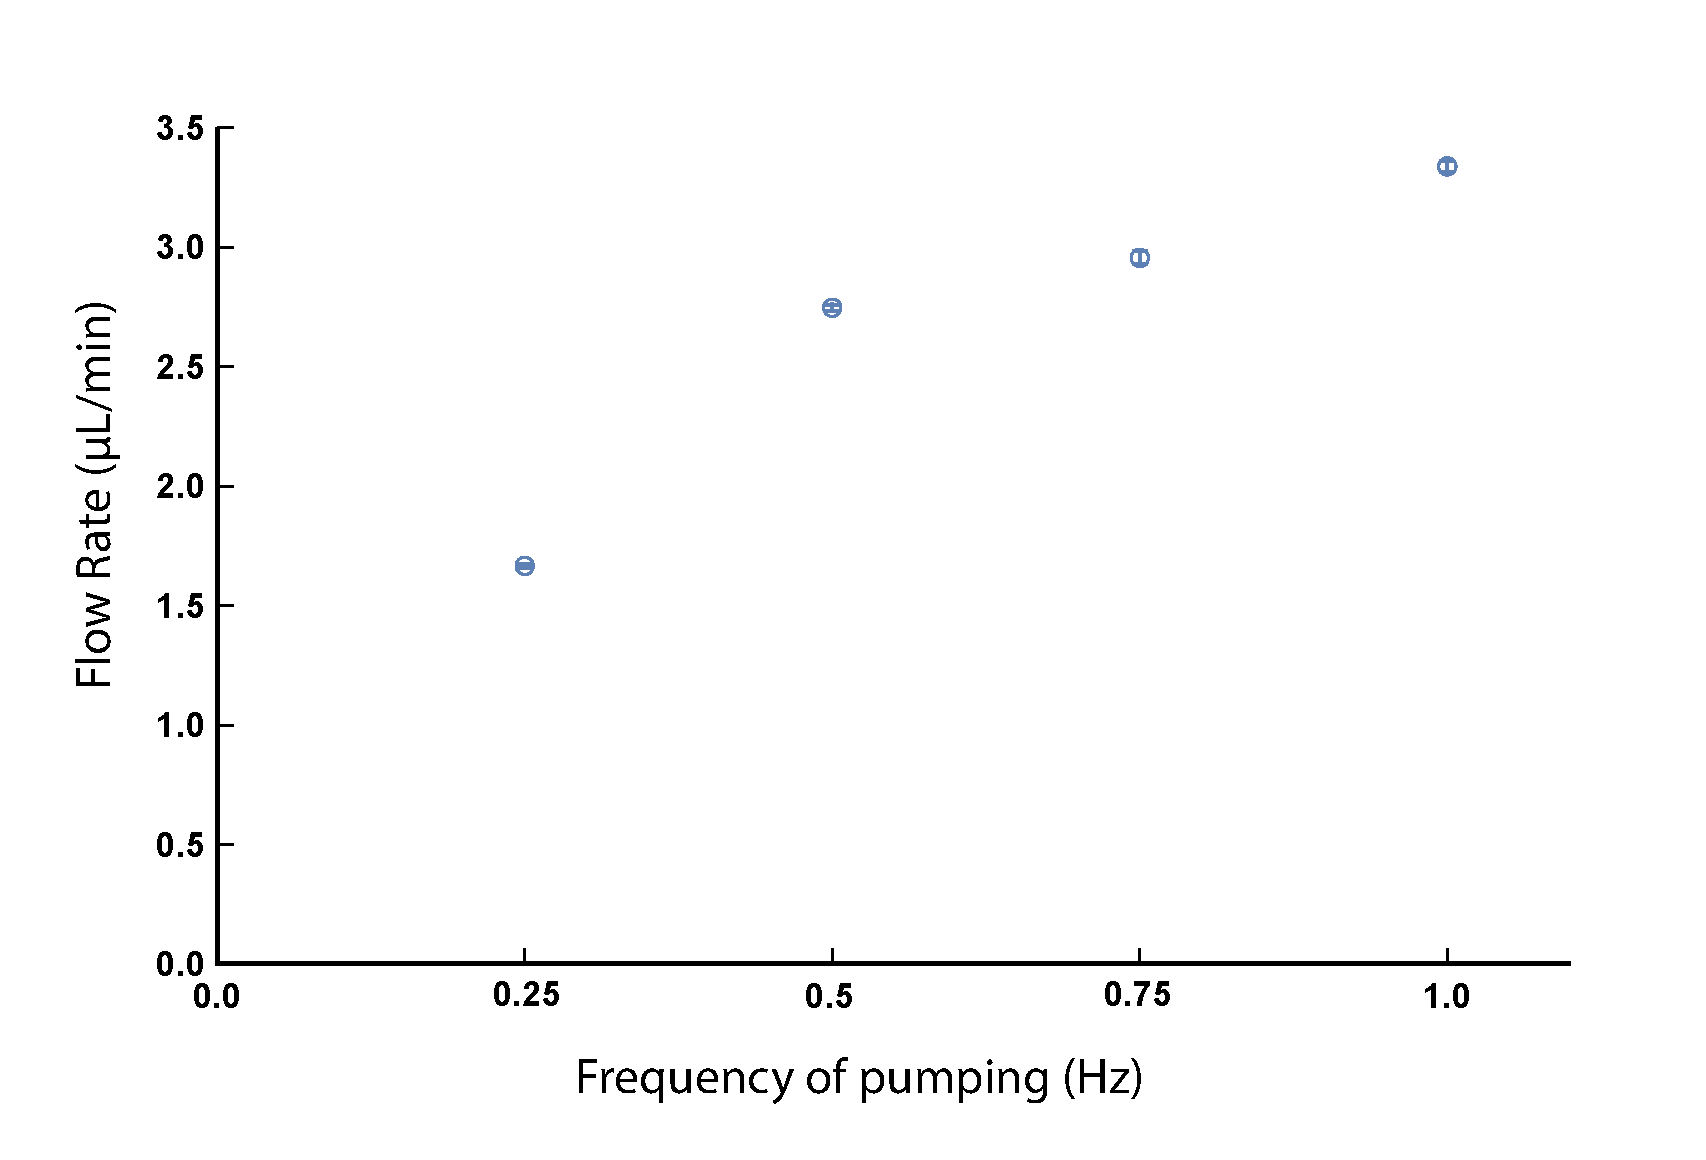
\includegraphics[height=8cm,keepaspectratio]{Flowratevsfreq.pdf}
  \caption{Flow rates produced by the pump at different frequencies.}
  \label{fig:FRvFGraph}
  \end{center}
\end{figure}

In \fig{fig:FRvFGraph}, the flow rate of the pump at varying frequencies is plotted. This
shows that the flow rate doesn't linearly depend on frequency, and seems to level off at higher
frequencies. When initially observing the gradient of the lines in \fig{fig:Graph}, the non-
linearity was attributed to inconsistencies in the tightening of the screws in the device.
However, the small error bars associated with the flow rates across three separate
experiments, each with at least one disassembly and reassembly of the device, it is now thought that the limit of the
pump rate is related to the elasticity of the membrane, and how fast it's able to 'snap
back' and re prime itself to pump in each valve.

\subsection{\textit{In situ} operation of the device}

\begin{figure}[h]
  \begin{center}
  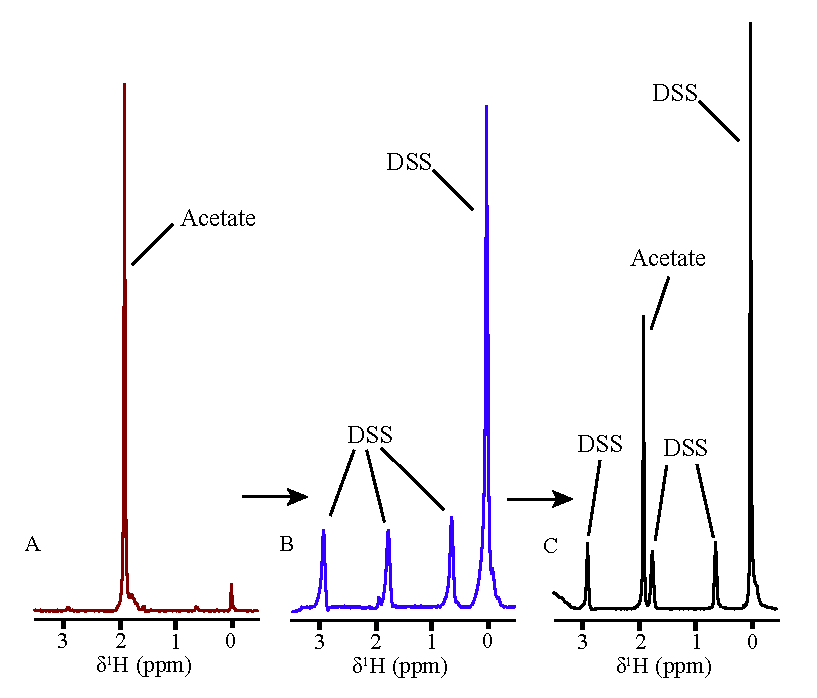
\includegraphics[height=12cm,keepaspectratio]{Acetate-DSS-stackplot-edit.pdf}
  \caption{NMR spectra recorded with 16 transients on a device containing 100mM Sodium
  acetate in the inner circuit and 100mM DSS in the outer circuit.}
  \label{fig:spectra}
  \end{center}
\end{figure}

In order to validate the pumps compatibility with NMR, the device was placed into a home
built transmission line probe inside a 500 MHz magnet. The arduino controller and solenoid valve
bank where secured outside the magnet and the 6 pressurised air lines fed in through the top of
the magnet. The device was then filled with 100mM sodium acetate in DI water (Sigma Aldrich) in
the inner circuit by attaching a syringe to inlet \textbf{B} in \fig{fig:Chip}. 100mM DSS in DI
water (Sigma Aldrich) was added to the outer circuit by syringing into inlet \textbf{A}. The sample chamber then contained only sodium acetate and all the initial signal should arise from this. The two fluid networks
were then connected using two short lengths of 1/16" outer diameter PTFE tubing by joining
\textbf{A} to \textbf{B} and \textbf{C} to \textbf{D}.

First, a spectra was collected of the chip after filling, A in \fig{fig:spectra}, using 16
transients and shows mainly the acetate signal at 1.9 ppm. The pump was then put into
the 'advance' state for 120 seconds which mean the valves are actuated in order to pump
liquid around both circuits. The pump then mixed in the inner circuit for 120 seconds
and a second spectra was recorded, B. This shows the 4 signals typical of DSS at 2.91
ppm, 1.75 ppm, 0.63 ppm and 0 ppm and very little acetate signal. Indicating that the
volume inside the NMR sensitive area has been almost entirely exchanged. Lastly the
pump again advanced and mixed for the same time as before producing the spectra shown
in C. Again, this spectrum is different. It shows all signals expected in abundance.
This points to mixing of the two substances facilitated by the peristaltic pump and serves
as proof, at least in principle, that an NMR compatible microfluidic peristaltic pump
capable of mixing liquids in a controllable manor has been presented here.

\section{Conclusions}

In conclusion, an NMR compatible; low dead volume microfluidic pump has been designed and
manufactured that works inside the bore of a high field magnet. The pump has shown
excellent linearity and stability in the long term as well as performing exchange, and
mixing, of two substances within the device inside a high field magnet. The present limitations
are that precise volume control has not yet been achieved. This is, however, thought to be linked
with the varied tightening of the screws of the 3D holder as well as the presence of bubbles
within the device. Another element that requires further probing is the non-linear dependence of
flow rate on frequency. My intuition is that this depends on the thickness of the PDMS layer
used
however further experimentation with varying thicknesses is needed. Potential future
applications
of this pump include: microfluidic protein binding experiments; \textit{in situ} liver slice
culture and metabolomics; and hyperpolarization experiments.
